%% 
%% Copyright 2007-2020 Elsevier Ltd
%% 
%% This file is part of the 'Elsarticle Bundle'.
%% ---------------------------------------------
%% 
%% It may be distributed under the conditions of the LaTeX Project Public
%% License, either version 1.2 of this license or (at your option) any
%% later version.  The latest version of this license is in
%%    http://www.latex-project.org/lppl.txt
%% and version 1.2 or later is part of all distributions of LaTeX
%% version 1999/12/01 or later.
%% 
%% The list of all files belonging to the 'Elsarticle Bundle' is
%% given in the file `manifest.txt'.
%% 

%% Template article for Elsevier's document class `elsarticle'
%% with numbered style bibliographic references
%% SP 2008/03/01
%%
%% 
%%
%% $Id: elsarticle-template-num.tex 190 2020-11-23 11:12:32Z rishi $
%%
%%
\documentclass[preprint,12pt]{elsarticle}

%% Use the option review to obtain double line spacing
%% \documentclass[authoryear,preprint,review,12pt]{elsarticle}

%% Use the options 1p,twocolumn; 3p; 3p,twocolumn; 5p; or 5p,twocolumn
%% for a journal layout:
%% \documentclass[final,1p,times]{elsarticle}
%% \documentclass[final,1p,times,twocolumn]{elsarticle}
%% \documentclass[final,3p,times]{elsarticle}
%% \documentclass[final,3p,times,twocolumn]{elsarticle}
%% \documentclass[final,5p,times]{elsarticle}
%% \documentclass[final,5p,times,twocolumn]{elsarticle}

%% For including figures, graphicx.sty has been loaded in
%% elsarticle.cls. If you prefer to use the old commands
%% please give \usepackage{epsfig}

%% The amssymb package provides various useful mathematical symbols
\usepackage{amssymb}
\usepackage{multirow}
\usepackage{lineno}
\usepackage[colorlinks,citecolor=black,linkcolor=black,urlcolor=black,bookmarks,bookmarksnumbered]{hyperref}
%% The amsthm package provides extended theorem environments
\usepackage{amsthm}
\usepackage{amsmath}

\newtheorem{theorem}{Theorem}[section]
\newtheorem{remark}[theorem]{Remark}
\newtheorem{corollary}{Corollary}[theorem]
\newtheorem{definition}{Definition}[section]

%% The lineno packages adds line numbers. Start line numbering with
%% \begin{linenumbers}, end it with \end{linenumbers}. Or switch it on
%% for the whole article with \linenumbers.
%% \usepackage{lineno}

\journal{Energy}

\begin{document}

\begin{frontmatter}

%% Title, authors and addresses

%% use the tnoteref command within \title for footnotes;
%% use the tnotetext command for theassociated footnote;
%% use the fnref command within \author or \address for footnotes;
%% use the fntext command for theassociated footnote;
%% use the corref command within \author for corresponding author footnotes;
%% use the cortext command for theassociated footnote;
%% use the ead command for the email address,
%% and the form \ead[url] for the home page:
%% \title{Title\tnoteref{label1}}
%% \tnotetext[label1]{}
%% \author{Name\corref{cor1}\fnref{label2}}
%% \ead{email address}
%% \ead[url]{home page}
%% \fntext[label2]{}
%% \cortext[cor1]{}
%% \affiliation{organization={},
%%             addressline={},
%%             city={},
%%             postcode={},
%%             state={},
%%             country={}}
%% \fntext[label3]{}

\title{Self-tunable approximated explicit MPC: Heat exchanger implementation and analysys}
%\title{Self-tunable approximated explicit MPC: Implementation on a heat exchanger with a non-symmetric behavior}

%% use optional labels to link authors explicitly to addresses:
%% \author[label1,label2]{}
%% \affiliation[label1]{organization={},
%%             addressline={},
%%             city={},
%%             postcode={},
%%             state={},
%%             country={}}
%%
%% \affiliation[label2]{organization={},
%%             addressline={},
%%             city={},
%%             postcode={},
%%             state={},
%%             country={}}

\author{Lenka Galčíková}
\author{Juraj Oravec}
\author{Petronela Belková}

\affiliation{organization={Slovak University of Technology in Bratislava, Faculty of Chemical and Food Technology, Institute of Information Engineering, Automation, and Mathematics,},%Department and Organization
            addressline={Radlinského 9}, 
            city={Bratislava},
            postcode={81237}, 
%            state={Slovakia},
            country={Slovakia}
}

\begin{abstract}
%max 250 words!
The tunable approximated explicit model predictive control (MPC) comes with the benefits of real-time tunability without the necessity of solving the optimization problem online. This paper provides a self-tunable technique that does not require any further tuning or interventions of the control engineer during operation. Based on the current operating conditions, the tuning parameter adjusts itself and scales the control input using linear interpolation. The adjustment of the tuning parameter depends on the reference value, which makes this strategy suitable for reference tracking problems. Furthermore, a novel technique for scaling the tuning parameter is proposed. It provides to exploit different ranges of the tuning parameter assigned to specified operating conditions. The self-tunable explicit MPC was implemented on a laboratory heat exchanger with nonlinear and non-symmetric behavior. To ensure offset-free control, the built-in integrator was included in the explicit MPC. The asymmetric behavior of the plant was compensated by tuning the controller's aggressivity, as the negativity or positivity of reference change was considered in the tuning process. The control performance decreased maximal overshoots/undershoots, integral square error, and settling time compared to control with only one controller. 
\end{abstract}

%%Graphical abstract
\begin{graphicalabstract}
%\includegraphics{grabs}
\end{graphicalabstract}

%%Research highlights
\begin{highlights}
% 3-5 highlights, every one should not exceed 85 characters including spaces
\item Self-tunable control technique does not need any intervention during control
\item Tuning based on the operating conditions compensates the nonlinear plant behavior
\item Implementation of the proposed tuning method on a laboratory heat exchanger 
\item Control performance improved compared to utilizing only one explicit MPC
\end{highlights}

\begin{keyword}
tunable explicit MPC \sep self-tunable technique \sep tuning parameter \sep heat exchanger \sep control performance
%% keywords here, in the form: keyword \sep keyword

%% PACS codes here, in the form: \PACS code \sep code

%% MSC codes here, in the form: \MSC code \sep code
%% or \MSC[2008] code \sep code (2000 is the default)

\end{keyword}

\end{frontmatter}

%% \linenumbers

%% main text
\section{Introduction}
\label{sec:introduction}
 
(len skopirovany text z jadra - hodil sa mi viac do Introduction, neskor mozno pouzijem) The benefit in form of lower computational complexity in the control phase comes hand in hand with a drawback. The size of the parametric solution may be so large, that it becomes impractical to utilize for two reasons: (i) memory footprint is higher than the available memory size of the control unit, (ii) the computational time associated with finding the optimal control action is higher than the available time period for control action implementation. Although this control strategy has its challenges, it is still very beneficial for practical usage for its benefits. 

\section{Preliminaries}
\label{sec:preliminaries}
In this section, the theoretical background necessary for this work is summarized. First, the explicit model predictive control is recalled. Next, the tunable technique of the approximated explicit model predictive control is introduced. Last but not least, the ideas of self-tunable technique of the approximated explicit MPC are presented.

\subsection{Explicit model predictive control}
\label{sec:eMPC}
Explicit model predictive control~\cite{Bemporad_automatica} represents a parametric solution of the model predictive control which makes it suitable for online implementation. As the explicit solution is available, it is not necessary to solve the optimization problem in every control step. As this work deals with practical implementation, let us consider the optimization problem in the following form:
\begin{subequations}
	\label{eq:mpc_problem}
	\begin{eqnarray}
		\label{eq:mpc_problem_cost}
		\min_{u_0,u_{1},\ldots,u_{N-1}} &~& \! \sum_{k=0}^{N-1} \! \left( (y_k-y_\mathrm{ref})^{\intercal} Q_\mathrm{y} (y_k-y_\mathrm{ref}) + u_{k}^{\intercal} R u_{k} + x_{\mathrm{I},k}^{\intercal} Q_\mathrm{x} x_{\mathrm{I},k} \right)  \\
		\label{eq:mpc_problem_prediction_model_x}
		\mathrm{s.t.\!:} &~& \widetilde{x}_{k+1} = \widetilde{A}\,\widetilde{x}_{k} + \widetilde{B}\,u_{k}, \\
		\label{eq:mpc_problem_prediction_model_y}
		&~& y_{k} = \widetilde{C}\,\widetilde{x}_{k}, \\
		\label{eq:mpc_problem_input_constraints}
		&~& u_{k} \in \mathcal{U}, \\
		\label{eq:mpc_problem_state_constraints}
		&~& y_{k} \in \mathcal{Y}, \\
		\label{eq:mpc_problem_initial_coindition}
		&~& \widetilde{x}_{0} = \theta, \\
		\label{eq:mpc_problem_k_range}
		&~& k = 0,1,\ldots, N-1,
	\end{eqnarray}
\end{subequations}

where $k$ denotes the step of the prediction horizon $N$. The parameter $\theta \in \Theta$ in Eq.~\eqref{eq:mpc_problem_initial_coindition} represents the initial condition of the optimization problem for which it is parametrically precomputed. Variables $\widetilde{x} \in \mathbb{R}^{n_{\widetilde{\mathrm{x}}}}$, $u \in \mathbb{R}^{n_{\mathrm{u}}}$, $y \in \mathbb{R}^{n_{\mathrm{y}}}$ are vectors of corresponding extended system states, control inputs and system outputs, respectively. The prediction model in~\eqref{eq:mpc_problem_prediction_model_x}--\eqref{eq:mpc_problem_prediction_model_y} has the form of extended linear time-invariant (LTI) system for given extended state matrix $\widetilde{A} \in \mathbb{R}^{n_{\widetilde{\mathrm{x}}} \times n_{\widetilde{\mathrm{x}}}}$, extended input matrix $\widetilde{B} \in \mathbb{R}^{n_{\widetilde{\mathrm{x}}} \times n_{\mathrm{u}}}$ and extended output matrix $\widetilde{C} \in \mathbb{R}^{n_{\mathrm{y}} \times n_{\widetilde{\mathrm{x}}}}$. The sets $\mathcal{U} \subseteq \mathbb{R}^{n_{\mathrm{u}}}$, $\mathcal{Y} \subseteq \mathbb{R}^{n_{\mathrm{y}}}$ are sets of physical constraints on inputs and outputs, respectively. The penalty matrix $Q_\mathrm{y} \in \mathbb{R}^{n_{\mathrm{y}} \times n_{\mathrm{y}}}$ penalizes the squarred control error, i.e., the deviation between the output and output reference value $y_\mathrm{ref}$. The matrix $R \in \mathbb{R}^{n_{\mathrm{u}} \times n_{\mathrm{u}}}$ penalizes the squarred value of control inputs. To obtain the offset-free control results, the built-in integrator was included in the state-space model, see e.q.~\cite{Ruscio_MPC_integral}. The value of integrator is also penalized in the cost function with the penalty matrix $Q_\mathrm{x} \in \mathbb{R}^{n_{\mathrm{y}} \times n_{\mathrm{y}}}$.

The model extended with the built-in integrator in~\eqref{eq:mpc_problem_prediction_model_x}--\eqref{eq:mpc_problem_prediction_model_y} can be rewritten as:
\begin{subequations}
	\begin{eqnarray} 
		\label{eq:mpc_extended_model_x} 
		\widetilde{x}_{k+1} &=& \begin{bmatrix} x_{k+1} \\ 	x_{\mathrm{I},k+1}\end{bmatrix} = \begin{bmatrix} A & \textit{0} \\ -T_\mathrm{s} C & I \end{bmatrix} \begin{bmatrix} x_{k} \\ x_{\mathrm{I},k} \end{bmatrix} + \begin{bmatrix} B \\ I \end{bmatrix} u_{k}, \\
		\label{eq:mpc_extended_model_y}
		y_k &=& \begin{bmatrix} C & \textit{0} \end{bmatrix} \begin{bmatrix} x_{k} \\ x_{\mathrm{I},k} \end{bmatrix},
	\end{eqnarray}
\end{subequations}

where $x_{\mathrm{I}} \in \mathbb{R}^{n_{\mathrm{y}}}$ is the integral of the control error, $T_\mathrm{s}$ denotes the sampling time and matrices $A$, $B$, $C$ are well-known linear time-invariant state-space matrices that form the extended model. Thanks to this extension and penalization in the cost function in Eq.~\eqref{eq:mpc_problem_cost}, not only the control error are penalized, but also its integral, which leads to similar results as incorporating integral part in PID controller.

Solving the MPC quadratic optimization problem in Eq.~\eqref{eq:mpc_problem} parametrically leads to explicit solution in the form of piece-wise affine control law consisting of $r$ critical regions:
\begin{eqnarray}
\label{eq:PWA_control_law}
u(\theta) = \left\{ 
\begin{matrix}
	F_{1} \, \theta + g_{1} & \mathrm{if} & \quad \theta \in \mathcal{R}_1, \\
	F_{2} \, \theta + g_{2} & \mathrm{else}\,\,\mathrm{if} &\quad \theta \in \mathcal{R}_2, \\
	\vdots & \\
	F_{r} \, \theta + g_{r} & \mathrm{else}\,\,\mathrm{if} & \quad \theta \in \mathcal{R}_{r}, \\
\end{matrix}
\right.
\end{eqnarray}
where $F_{i}$ and $g_{i}$ respectively are the slope and affine section of the corresponding control law. The piece-wise affine function from Eq.~\eqref{eq:PWA_control_law} is stored and used in the online, i.e., control phase. Based on identifying the critical region where the parameter $\theta$ belongs, the optimal control input is calculated based on the associated control law.

Note, many other formulations of the optimization problems are elaborated, mainly in the terms of cost functions. Also, the incremental (velocity) formulation of the state-space model is common, but leads to further extendsion of the vector of parameters $\theta$ and therefore the explicit MPC complexity increases. Another option for offset-free tracking is also disturbance observer. For such an overview see e.g. ...TODO. 
Klauco reference governors? minimovka zdroje + dizertacka str.33
      

\subsection{Tunable explicit model predictive control}
\label{sec:tunable}
The aggressivity of the controller and whole nature of the control can be influenced by tuning the penalty matrices in the optimization problem~\eqref{eq:mpc_problem}. When the optimization problem is precomputed offline to obtain the parametric solution, it is not possible to tune the controller afterwards. As the operation conditions and demands on controller setup may differ throughout control, the ability to adjust the controller aggressivity can be very beneficial.

The idea of approximated tunable explicit MPC comes from the work ~\cite{Klauco_tunable}, where the control action is calculated based on linear interpolation between two boundary control actions. These control actions result from evaluating two boundary explicit MPCs. The boundary explicit controllers have the same structure and setup, except one of the penalty matrices -- the tuned one. The boundary matrices are diagonal square matrices such that $\lambda_{i,\mathrm{L}} \le \lambda_{i,\mathrm{U}}$, $\forall i = 1,\dots,s$, where $\lambda$ denotes the vector of penalty matrix eigenvalues, $L$ and $U$ denote the lower and upper boundary setup respectively, and $s$ is the rank of the tuned penalty matrix.

When considering the penalty matrices from cost function~\eqref{eq:mpc_problem_cost}, the penalty matrices are scaled in the following way:
\begin{subequations}
	\label{eq:tunable_matrices}
	\begin{eqnarray}
		\label{eq:tunable_R}
		&~& R = (1-\rho)R_\mathrm{L} + \rho R_\mathrm{U}, \\
		\label{eq:tunable_Qx}
		&~& Q_\mathrm{x} = (1-\rho)Q_\mathrm{x,L} + \rho Q_\mathrm{x,U}, \\
		\label{eq:tunable_Qy}
		&~& Q_\mathrm{y} = (1-\rho)Q_\mathrm{y,L} + \rho Q_\mathrm{y,U},
	\end{eqnarray}
\end{subequations}

where $\rho$ represents the tuning parameter and $0 \le \rho \le 1$ holds. Based on~\eqref{eq:tunable_matrices}, it is possible to choose online any controller setup from the lower to the upper boundary of the tuned matrix. Note, it is practical to tune only one matrix, i.e., to store only two controllers corresponding to the boundary matrices. To determine which penalty matrix should be tuned, it is suggested to examine the control results subject to the specific system and to try systematic tuning of all the penalty matrices.

When the tuning parameter $\rho$ is determined based on the current control conditions, the optimal control action is evaluated using the two optimal controllers. Based on the boundary control actions, the interpolated, i.e., tuned control action is calculated:
\begin{subequations}
	\begin{eqnarray}
		\label{eq:tunable_u}
		u = (1-\rho)u_\mathrm{L} + \rho u_\mathrm{U},
	\end{eqnarray}
\end{subequations}

where $u_\mathrm{L}$ and $u_\mathrm{U}$ denote the optimal control actions from the lower and upper boundary controller respectively. The tuning of the controller online comes with a cost of storing and evaluating two explicit controllers. Nevertheless, the ability to tune the controller may be more important in many practical applications.

Note, the concept of explicit MPC tuning can be applied also to other MPC formulations, based on the current specific needs. In this paper, the penalty matrices of cost function~\eqref{eq:mpc_problem_cost} are considered, as it is necessary to satisfy offset-free reference tracking.

\begin{remark}
	If stability guarantee and recursive feasibility is required, it is suggested to follow the instructions from \cite{Oravec_tunable}. In order to satisfy the requirements, the study introduces a procedure of choosing the terminal penalty and terminal set in the two boundary controllers. 
\end{remark}

\subsection{Self-tunable explicit model predictive control}
\label{sec:self_tunable}
The advantage of tunable controller brings a question of how to design the logic of setting the tuning parameter $\rho$. In this section, the idea of online self-tuning is summarized~\cite{self_tunable}. The concept of self-tuning provides the possibility to adjust the aggressiveness of the controller without the necessity to intervene and tune the penalty matrices during control. 

The need for real-time controller tuning often arises from tracking a time-varying reference. The work~\cite{self_tunable} focuses on adjusting the penalty matrix when the reference value is changed. The further the reference value is from the steady state, the more aggressive controller is tuned. The idea behind the suggested scaling liest in compensation of the nonlinear behavior of the system.  

The procedure of tuning the controller is based on evaluating the difference between the reference and the steady state, and using this deviation to scale the value of control action. First, the maximal absolute value of reference which can be set during control is defined. This value can be determined based on the general knowledge of future reference values. Another suggestion is to set the maximal deviation $d_{\max}$ simply based on the constraints on system outputs: 
\begin{eqnarray}
	\label{eq:d_max}
	d_{\max} = \max(\vert y_{\min} \vert, y_{\max}),
\end{eqnarray}

where $y_{\min}$ and $y_{\max}$ are respectively lower and upper bound on the output variable. Using the information about the maximal possible deviation $d_{\max}$, the tuning parameter $\rho$ can be calculated as the ratio between the current reference value and the maximal deviation:  

\begin{eqnarray}
	\label{eq:rho_self_tunable}
	\rho = \frac{\vert y_{\mathrm{ref}} \vert}{d_{\max}}.
\end{eqnarray}

Based on Eq.~\eqref{eq:rho_self_tunable}, the property $0 \le \rho \le 1$ holds, as $\vert y_{\mathrm{ref}} \vert \le d_{\max}$. As a result, the parameter $\rho$ represents a way how to normalize the deviation from steady state and is exploited to scale the penalty matrix or at the end of the day, the control action. 

When considering tuning the control action based on Eq.~\eqref{eq:tunable_u}, a higher value of tuning parameter $\rho$ leads to approaching the upper boundary controller and vice versa. When tuning e.g. the matrix $Q_\mathrm{y}$ penalizing the control error, a higher ratio $\rho$ would lead to more aggressive control actions. When controlling to the reference values closer to the steady state, the parameter $\rho$ decreases and the control becomes sluggish.

\begin{remark}
	The parameter $d_{\max}$ is vector in general, as it depends on the size of system outputs. If $d_{\max}$ is scalar, the parameter $\rho$ is scalar as well and can be directly utilized to scale the control action. If multiple outputs are controlled, it is suggested to calculate the tuning parameter based on the maximal ratio:
	\begin{eqnarray}
		\label{eq:rho_max}
		\rho = \max \left( \frac{\vert y_{\mathrm{ref}} \vert}{d_{\max}} \right).
	\end{eqnarray}	
\end{remark}

Note, the relations \eqref{eq:rho_self_tunable} and \eqref{eq:rho_max} operate with the absolute value of the reference. It is not taken into account, whether the reference change was positive or negative, i.e., whether it changed upwards or downwards. As many plants have non-symmetric behavior, the positivity or negativity of the reference change could be considered in the controller tuning to improve the control performance.
    

\section{Methodology}
\label{sec:methodology}
This section extends the ideas of self-tunable explicit MPC in order to improve the control performance. First, a different way of tuning parameter calculation is introduced. Furthermore, an extended self-tunable technique is presented to scale the tuning parameter for applications, when it is beneficial to exploit a specific range of the tuning parameter in different operating conditions. 


\subsection{Tuning parameter based on the size of reference change}
\label{sec:self_tunable_delta_ref}
The approach of self-tunable explicit MPC in~\cite{self_tunable} suggested tuning based on the reference value distance from the steady state. The aim is to compensate the nonlinear behavior of system, when using a simple linear prediction model. This work provides another way of the tuning parameter calculation based on the size of reference change. When different sizes of reference step changes are made and the behavior of the closed-loop system is varying, it can be beneficial to inclue the size of the reference step change into the tuning procedure.

In this approach, the aggressivity is adjusted based on the ratio between the reference step change and the maximal reference step change that can be set during control operation:
\begin{eqnarray}
	\label{eq:rho_delta_ref}
	\rho = \frac{\vert \Delta_{\mathrm{ref}} \vert}{d_{\max}},
\end{eqnarray} 

where $\Delta_{\mathrm{ref}} = y_{\mathrm{ref},k}-y_{\mathrm{ref},k-1}$ is the size of the reference change. The denominator of Eq.~\eqref{eq:rho_delta_ref} is changed as well. In contrast to the maximal deviation from the steady state in Section~\ref{sec:self_tunable}, this approach introduces $d_{\max}$ as the maximal possible reference step. 
Analogously to the original approach, the maximal reference step can be set based on the general knowledge of future reference values. Another option is to exploit the information about the system constraints and set the parameter $d_{\max}$ according to Eq.~\eqref{eq:d_max}. 
 
Note, only absolute value of $\Delta_{\mathrm{ref}}$ and $d_{\max}$ are considered in this procedure to ensure $\rho \ge 0$. 

\begin{remark}
	The tuning parameter $\rho$ should be updated only when the reference changes. Updating the tuning parameter in the control steps when $\Delta_{\mathrm{ref}} = 0$ would lead to using tuning parameter $\rho$ with zero value, i.e., the control input would correspond to one boundary controller and would not be scaled.
\end{remark}


\subsection{Self-tunable technique for systems with asymmetric behavior}
\label{sec:self_tunable_rho_scaling}
\noindent TODO: co ak nepriama umera? \\
TODO: remark na nelinearnu interpolaciu \\
TODO: zovseobecnit na viac usekov intervalu? \\

This paper provides further extension of the self-tuning method proposed in~\cite{self_tunable}. The suggested technique of tuning is suitable e.g. for systems with non-symmetric behavior, but can be used in any application, where ,,simple" tuning in the whole range of tuning parameter $\rho$ is not sufficient.

The tuning method is based on splitting the interval of the tuning parameter $\rho$ in order to utilize different parts of the interval in different operating conditions. The adjusted tuning parameter $\widetilde{\rho}$ is then utilized to scale the control input according to Eq.~\eqref{eq:tunable_u} instead of the original value of tuning parameter $\rho$.     

\begin{definition}
	If the tuning parameter is scaled in the first part of the interval, i.e., $\langle 0, \rho_{\mathrm{s}} \rangle$, where $\rho_{\mathrm{s}}$ is the splitting value of the tuning parameter, the following relation is used to adjust the tuning parameter:
	\begin{eqnarray}
		\label{eq:rho_up}
		\widetilde{\rho} = \rho_{\mathrm{s}} \rho.
	\end{eqnarray}
\end{definition}

\begin{corollary}
	The following outcomes result from Eq.~\eqref{eq:rho_up}. If $\rho=0$, then $\widetilde{\rho} = 0$. When considering the other extreme, i.e., $\rho=1$, then $\widetilde{\rho} = \rho_{\mathrm{s}}$. In such way, the parameter $\rho$ can be scaled in the first part of the interval up to the splitting value. Note, as the relation in Eq.~\eqref{eq:rho_up} is linear and $0 \le \rho \le 1$ holds, for $\widetilde{\rho}$ it is impossible to acquire other values than in the given interval of parameter $\rho$.   
\end{corollary}

\begin{definition}
	If the tuning parameter is scaled in the second part of the interval, i.e., $\langle \rho_{\mathrm{s}}, 1 \rangle$, the following relation is used to adjust the tuning parameter:	
	\begin{eqnarray}
		\label{eq:rho_down}
		\widetilde{\rho} = (1-\rho_{\mathrm{s}}) \rho + \rho_{\mathrm{s}}.
	\end{eqnarray}
\end{definition}

\begin{corollary}
	The following outcomes result from Eq.~\eqref{eq:rho_down}. When $\rho=0$, $\widetilde{\rho} = \rho_{\mathrm{s}}$. When considering the other extreme, i.e., $\rho=1$, then $\widetilde{\rho} = 1$. In such way, the parameter $\rho$ can be scaled in the second part of the interval from to the splitting value up to 1. Note, as the relation in Eq.~\eqref{eq:rho_down} is linear and $0 \le \rho \le 1$ holds, for $\widetilde{\rho}$ it is impossible to acquire other values than in the given interval of parameter $\rho$.
\end{corollary}

The advantage of the proposed method remains in the self-tuning of the controller as in the approach from Section~\ref{sec:self_tunable}. Nevertheless, it is required to determine the splitting value of the tuning parameter $\rho_{\mathrm{s}}$ and assign the parts of the interval to the associated operating conditions.

\begin{remark}
	Note, the suggested scaling method is suitable also for online MPC, as the optimization problem is solved in every control step. Therefore, it is possible to include the controller tuning in the procedure of computing the optimal control input. It should be also noted that with updating penalty matrices, the optimization problem has to be rebuilt into a form suitable for a solver, so sufficient computational time is required.  
\end{remark}

\section{Results and discussion}
\label{sec:results}

In this section, the results of the proposed tuning method are presented on an experimental implementation. The tuning strategy utilizes tuning parameter based n the size of reference change (Section~\ref{sec:self_tunable_delta_ref}) and the scaling of tuning parameter based on splitting the interval of the parameter and assigning the interval parts to specific operating conditions (Section~\ref{sec:self_tunable_rho_scaling}).

The plant on which the control was implemented is a laboratory liquid-to-liquid plate heat exchanger Armfield Process Plant Trainer PCT23~\cite{pct23}, see Fig.~\ref{fig:HE}. The cold feed as well as heating medium are transported to the heat exchanger by two peristaltic pumps. The flow rate of the feed is constant, while the aim is to track the reference value of its temperature. Therefore, the controlled output is the feed temperature $T$ at the outlet of the heat exchanger and the control input is the voltage $U$ corresponding to the power of the heating medium pump. The voltage is set in percentage, while it is constrained from 20\% to 100\%. As the heat exchange is a nonlinear and non-symmetric process~\cite{Liptak}, this heat exchanger represents a suitable candidate for the presented controller tuning strategy.  

The matrices of the linear state-space model of the plant, discretized with sampling time $T_\mathrm{s}$ = 1\,s, are
\begin{subequations}
	\label{eq:model_A_B} 
	\begin{eqnarray}
		A&=&\begin{bmatrix}
			0.839
		\end{bmatrix}, \\
		B&=&\begin{bmatrix}
			0.039
		\end{bmatrix}, \\
		C&=&\begin{bmatrix}
			1
		\end{bmatrix}, \\
		D&=&\begin{bmatrix}
			0
		\end{bmatrix}.
		\end{eqnarray}
\end{subequations}

The constraints are considered in the terms of control inputs, i.e.
\begin{eqnarray}
\label{eq:u_const}
	-15\% \le u \le 65\%.
\end{eqnarray}

Note, the variable $u$ represents the control inputs in the deviation form. The values of feed temperature and voltage of the heating medium pump corresponding to zero steady state are respectively $T^\mathrm{s}$~=~35 $^{\circ}\mathrm{C}$ and $U^\mathrm{s}$~=~35\%.

The penalty matrices of the problem Eq.~\eqref{eq:mpc_problem} were systematically tuned and the corresponding control was implemented on the laboratory heat exchanger for every MPC setup. The aim was to determine, which penalty matrix will be the tuned one. Based on observations, the most significant effect on the control trajectories had tuning the penalty matrix $Q_\mathrm{y}$, while still preserving a satisfactory control performance, i.e., without steady-state control error and significant oscillations around the setpoint. The boundary values of matrix $Q_\mathrm{y}$ were tuned as $Q_\mathrm{y, L}$ = 100 and $Q_\mathrm{y, U}$ = 1000. The built-in integrator was penalized with $Q_\mathrm{x}$ = 1 and the control input with $R$ = 10. The prediction horizon $N$ was 20 steps long. The explicit model predictive controllers were constructed in MATLAB R2020b using the Multi-Parametric Toolbox 3~\cite{mpt_conf}. 
The controllers were implemented to track a time-varying reference. For the first 200 seconds, the system was in the steady state. After that, the reference changed its value twice upwards and twice downwards. The reference changes also acquired different sizes in order to examine the proposed tuning method as it is dependent on the size of the reference step change. The control results for both control setups are compared in Fig.~\ref{fig:CV_boundaries} for the controlled outputs, and in Fig.~\ref{fig:MV_boundaries} for the control inputs.
    

\begin{figure}
	\begin{center}
		\includegraphics[width=0.8\textwidth]{images/HE}
		\caption[Heat exchanger Armfield Process Plant Trainer PCT23]{Laboratory heat exchanger Armfield Process Plant Trainer PCT23: feed pump\,(1), heating medium pump\,(2), feed tanks\,(3), heater for heating medium\,(4), heat exchanger\,(5).}
		\label{fig:HE}
	\end{center}
\end{figure}

\begin{figure}
	\begin{center}
		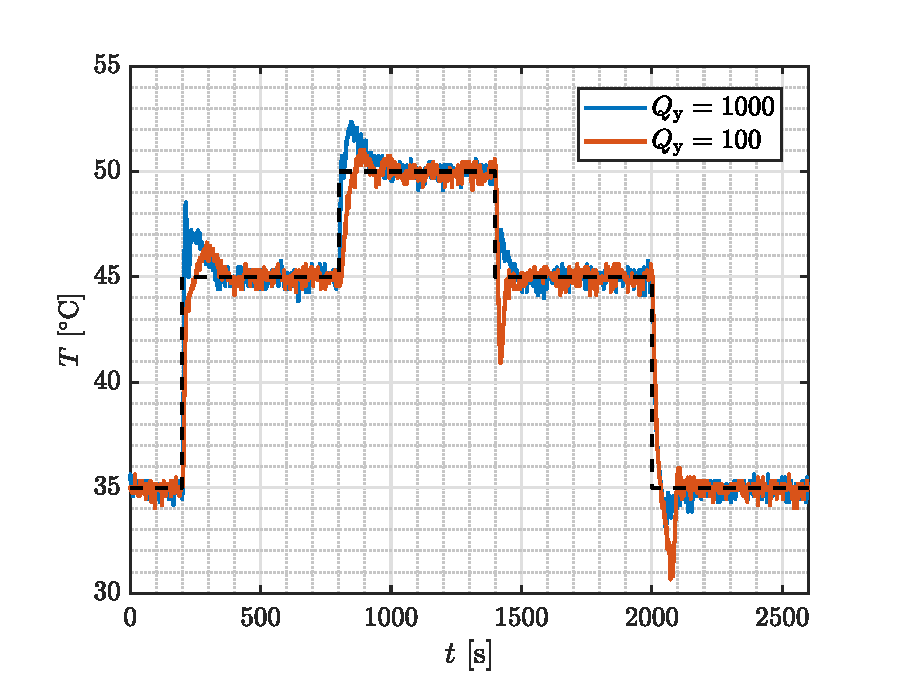
\includegraphics[width=0.8\textwidth]{images/CV_boundaries}
		\caption{Controlled output trajectory for two boundary controllers. The solid lines represent the controlled temperature and the dashed line represents the reference value.}
		\label{fig:CV_boundaries}
	\end{center}
\end{figure}

\begin{figure}
	\begin{center}
		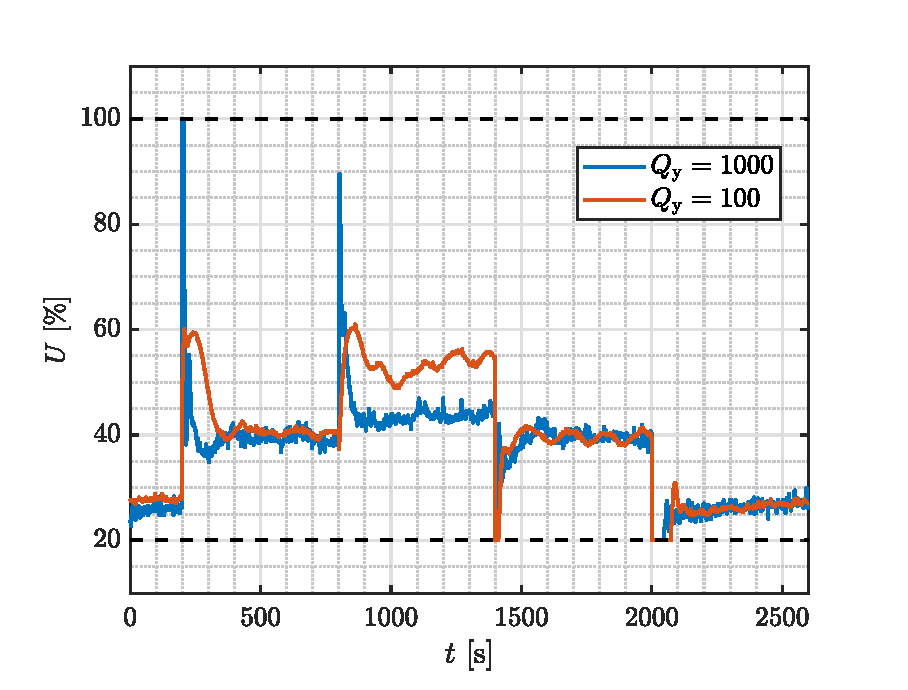
\includegraphics[width=0.8\textwidth]{images/MV_boundaries}
		\caption{Control input trajectory for two boundary controllers. The solid lines represent the voltage and the dashed lines represent the constraints.}
		\label{fig:MV_boundaries}
	\end{center}
\end{figure}

The trajectories in Fig.~\ref{fig:CV_boundaries} show the non-symmetric nature of controlling the process of heat exchange mainly when observing the overshoots and undershoots. When applying the control associated with the lower bound $Q_\mathrm{y, L}$, significant undershoots are present when tracking the reference downwards, i.e., when the reference change is negative. On the contrary, when implementing the controller associated with $Q_\mathrm{y, U}$, the undershoots are negligible, but significant overshoots can be seen when tracking the reference upwards.

These observations form the base for the strategy of self-tuning the penalty matrix $Q_\mathrm{y}$. The strategy follows the ideas summarized in Section~\ref{sec:self_tunable_new}. Utilizing the boundary controller with the penalty matrix $Q_\mathrm{y,L}$ is preferred when the reference changes upwards. On the contrary, the controller associated with $Q_\mathrm{y,U}$ is preferred in control with negative reference changes. The splitting value of the tuning parameter was chosen in the middle of the interval, i.e., $\rho_{\mathrm{s}} = 0.5$. The last parameter that needed to be set was the maximal possible size of the reference step change $d_{\max}$, which was set to $15^{\circ}\mathrm{C}$. 

The control results of the selt-tunable technique compared to the boundary controllers can be seen in Fig.~\ref{fig:CV} for the controlled outputs, and in Fig.~\ref{fig:MV} for the control inputs. It can be seen that the tuned controller combined the benefits of the two boundary controllers. The overshoots and undershoots were reduced, as in the first half of control the penalty matrix $Q_\mathrm{y}$ acquired value from the first half of the penalty interval. When tracking the reference with negative change, the penalty matrix acquired the values from the second half of the interval, i.e., closer to the upper bound $Q_\mathrm{y,U}$. 
The similarity with the boundary controllers can be seen also on the control inputs trajectory. Note, the constraints on the input variable were satisfied as they were scaled using linear interpolation based on the boundary controllers which are constructed considering the contraints. 

TODO: what about state constraints?


\begin{figure}
	\begin{center}
		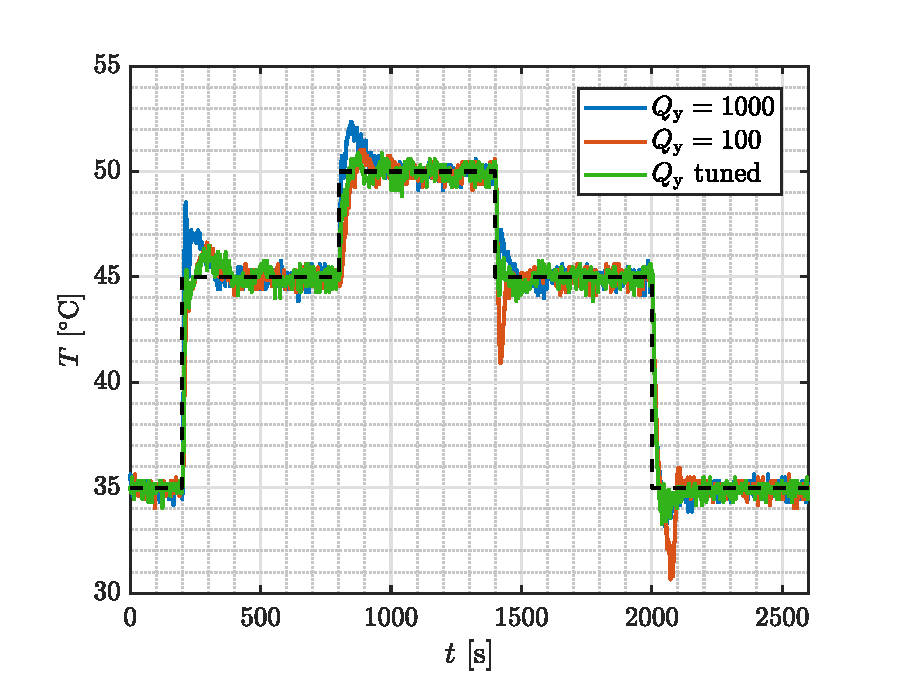
\includegraphics[width=0.8\textwidth]{images/CV}
		\caption{Controlled output trajectory for two boundary controllers and the tuned one. The solid lines represent the controlled temperature and the dashed line represents the reference value.}
		\label{fig:CV}
	\end{center}
\end{figure}

\begin{figure}
	\begin{center}
		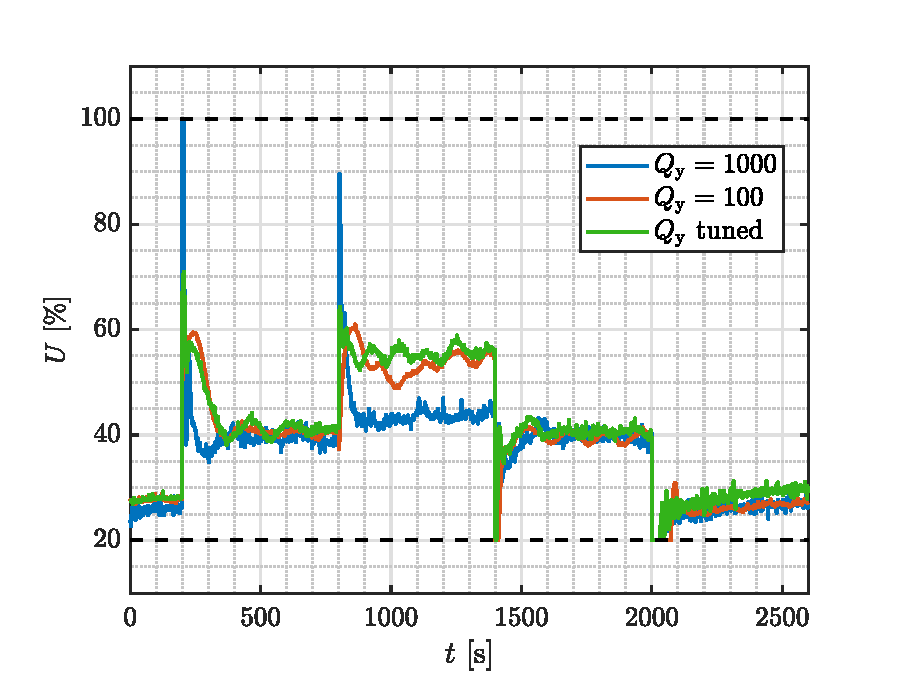
\includegraphics[width=0.8\textwidth]{images/MV}
		\caption{Control input trajectory for two boundary controllers and the tuned one. The solid lines represent the voltage and the dashed lines represent the constraints.}
		\label{fig:MV}
	\end{center}
\end{figure}

The control performance was also investigated quantitatively. The Table~\ref{tab:control_performance} summarizes the evaluated control performance criteria for the tuned and two boundary controllers. The control performance is evaluated for every reference step change respectively. The criteria are integral square error $ISE$, maximal overshoot/undershoot $\sigma_{\mathrm{max}}$, settling time $t_{\epsilon}$ for 5\%-neighbourhood of the reference value, and the volume of the heating medium utilized for the corresponding control. To provide better readability of the results, the best (i.e. minimal) values are written in bold. 

\begin{table}[h!]
	\begin{center}
		\caption{Control performance criteria.}
		\label{tab:control_performance}
		\begin{tabular}{c|c|c|c|c|c} 
			Reference step change & $Q_\mathrm{y}$ & $ISE$ [$^{\circ}\mathrm{C}^2$\,s] & $\sigma_{\mathrm{max}}$\,[\%] & $t_{\epsilon}$\,[s] & $V$\,[l] \\
			\hline
			\multirow{2}{*}{1} & 1000 & 714 & 33.50 & 16.5 & \textbf{2.12} \\
			    & 100 & 867 & 16.65 & 12.5 & 2.36 \\ 
			    & tuned & \textbf{678} & \textbf{15.19} & \textbf{9.5} & 2.38 \\ 
			\hline
			\multirow{2}{*}{2} & 1000 & 365 & 47.20 & \textbf{5} & \textbf{2.49} \\
			    & 100 & 606 & 23.25 & 26.5 & 3.19 \\ 
			    & tuned & \textbf{248} & \textbf{19.13} & 9.5 & 3.35 \\ 
			\hline
		    \multirow{2}{*}{3} & 1000 & 245 & \textbf{18.92} & \textbf{6.5} & \textbf{2.00} \\
				& 100 & 398 & 79.64 & 31 & \textbf{2.00} \\ 
				& tuned & \textbf{186} & 24.59 & \textbf{6.5} & 2.10 \\ 
			\hline
			\multirow{2}{*}{4} & 1000 & 1024 & 18.43 & 22.5 & 0.94 \\
				& 100 & 1402 & 41.87 & 90 & \textbf{0.93} \\ 
				& tuned & \textbf{967} & \textbf{16.49} & \textbf{18.5} & 1.10  
		\end{tabular}
	\end{center}
\end{table}

It can be seen in Table~\ref{tab:control_performance}, that real-time tuning of the controller helped to improve two to three criteria when tracking each reference value. The cost for this is the energy associated with control. Although the integral square error, maximal overshoot/undershoot and settling time decreased, the volume of consumed heating medium did not. Nevertheless, the average deterioration in the terms of consumed heating medium is approximately~17\%. 

The improvement or deterioration in percentage of using the tunable controller relative to the second best setup is summarized in Table~\ref{tab:improvement} for every reference step change separately. The negative numbers represent deterioration compared to the best controller setup in the corresponding reference tracking. 

\begin{table}[h!]
	\begin{center}
		\caption{Improvement or deterioration of the control performance in percentage.}
		\label{tab:improvement}
		\begin{tabular}{c|c|c|c|c} 
			Reference step change & $ISE$ & $\sigma_{\mathrm{max}}$ & $t_{\epsilon}$ & $V$ \\
			\hline
			1 & 5.04 & 8.77 & 24.00 & -12.26 \\ 
			\hline
			2 & 32.05 & 17.72 & -90.00 & -34.54 \\ 
			\hline
			3 & 24.08 & -29.97 & 0 & -4.48 \\ 
			\hline
			4 & 5.57 & 10.53 & 17.78 & -18.28  
		\end{tabular}
	\end{center}
\end{table}

It can be seen that implementing a tunable controller leads to improved control performance in many criteria. Utilizing a controller with a scalable aggressivity according to the operating conditions leads in general to higher accuracy, lower overshoot and faster achieving the reference value. %It should be also noted that the deterioration of every criterium is calculated subject to the best out of \textit{two} other controllers. It follows that the evaluation is strict as in practice only one controller would be available.
Although the volume of the heating medium is not saved in this control scenario, the improved control performance may lead to other benefits. 

TODO: krajsie skomentovat vyhody zlepsenia kvality riadenia

\section{Conclusion}
\label{sec:conclusion}
This paper deals with the experimental implementation of tunable approximated explicit model predictive control and provides a technique for self-tuning controller design. Based on the current reference value, the tuning parameter is scaled using linear interpolation. The previously published paper related to the self-tunable explicit MPC suggested tuning based on the distance of the reference value from the steady state. This paper presents a novel idea of tuning based on the size of reference step change. The tuning procedures aim to compensate for the nonlinear behavior of the controlled system. The tuning parameter is updated when the reference changes. It is calculated as the ratio between the size of the reference change and the maximal possible size of the reference change, which is specified before operation. Another novel contribution comes with splitting the interval of tuning parameter into two ranges, while both ranges are assigned to different operating conditions. The proposed method is implemented on a laboratory heat exchanger with nonlinear and non-symmetric behavior. The non-symmetry makes the plant a suitable candidate for splitting the interval of the tuning parameter. The decision criterium is negativity or positivity of reference change. When the reference changed upwards, the control input was tuned in the first part of the interval and approached the boundary controller associated with the lower bound on the penalty matrix. On the contrary, when the reference changed downwards, the control input was tuned to approach the control input from the boundary controller with the upper bound on the penalty matrix. To investigate the control results properly, the control performance was evaluated quantitatively. Compared to control with only one controller, the self-tunable technique helped to decrease the maximal overshoots/undershoots, integral square error, and settling time.

\section*{Acknowledgements}
This research is funded by the European Union’s Horizon Europe under grant no. 101079342 (Fostering Opportunities Towards Slovak Excellence in Advanced Control for Smart Industries). The authors gratefully acknowledge the contribution of the Scientific Grant Agency of the Slovak Republic under the grants 1/0545/20, 1/0297/22, the Slovak Research and Development Agency under the project APVV-20-0261. 

\section*{Nomenclature}

\subsection{Abbreviations}
\noindent  \textit{MPC}: model predictive control \\
\textit{ISE}: integral square error \\
\textit{LTI}: linear time-invariant \\

\subsection{Symbols}
\noindent $A$: system state matrix \\
$\widetilde{A}$: extended system state matrix \\
$B$: system input matrix \\
$\widetilde{B}$: extended system input matrix \\
$C$: system output matrix \\
$\widetilde{C}$: extended system output matrix \\
$d_{\max}$: maximal deviation from the steady state \\
TODO: odlisit max size of reference step change \\
$F$: slope of the affine control law \\
$g$: section of the affine control law \\
$I$: identity matrix \\	
$k$: step of the prediction horizon \\
$N$: prediction horizon \\
$n_{\mathrm{u}}$: size of system inputs \\
$n_{\mathrm{y}}$: size of system outputs \\
$n_{\widetilde{\mathrm{x}}}$: size of extended system states \\
$Q_{\mathrm{x}}$: penalty matrix of the built-in integrator \\
$Q_{\mathrm{x,L}}$: lower bound on the penalty matrix of the built-in integrator \\
$Q_{\mathrm{x,U}}$: upper bound on the penalty matrix of the built-in integrator \\
$Q_{\mathrm{y}}$: penalty matrix of the control error \\
$Q_{\mathrm{y,L}}$: lower bound on the penalty matrix of the control error \\
$Q_{\mathrm{y,U}}$: upper bound on the penalty matrix of the control error \\
$R$: penalty matrix of system inputs \\
$R_{\mathrm{L}}$: lower bound on the penalty matrix of system inputs \\
$R_{\mathrm{U}}$: upper bound on the penalty matrix of system inputs \\
$\mathcal{R}$: critical region \\
$\mathbb{R}$: Euclidean space of real numbers \\
$t$: time, s \\
$t_{\epsilon}$: settling time, s \\
$T$: temperature, $^{\circ}\mathrm{C}$ \\
$T_{\mathrm{s}}$: sampling time, s \\
$T^{\mathrm{s}}$: steady state of temperature, $^{\circ}\mathrm{C}$ \\
$u$: control inputs \\
$u_{\mathrm{L}}$: control inputs asscociated with the lower boundary controller\\
$u_{\mathrm{U}}$: control inputs asscociated with the upper boundary controller\\
$U$: voltage, \% \\
$U^{\mathrm{s}}$: steady state of voltage, \% \\
$\mathcal{U}$: set of control inputs \\
$V$: volume of heating medium, l \\
$x$: system states \\
$\widetilde{x}$: extended system states \\
$x_{\mathrm{I}}$: system states corresponding to the built-in integrator \\
$y$: system outputs \\
$y_\mathrm{\max}$: maximal value of system outputs \\
$y_\mathrm{\min}$: minimal value of system outputs \\
$y_\mathrm{ref}$: reference value of system outputs \\	
$\mathcal{Y}$: set of system outputs \\
\textit{0}: zero matrix

\subsection{Greek letters}
\noindent $\Delta_\mathrm{ref}$: size of the reference change, $^{\circ}\mathrm{C}$ \\
$\rho$:	tuning factor \\
$\widetilde{\rho}$: scaled tuning factor \\
$\rho_{\mathrm{s}}$: splitting value of the tuning factor \\
$\sigma_{\max}$: maximal overshoot, \% \\
$\theta$: parameter of optimization problem \\
$\Theta$: set of parameter values


%% The Appendices part is started with the command \appendix;
%% appendix sections are then done as normal sections
%% \appendix

%% \section{}
%% \label{}

%% If you have bibdatabase file and want bibtex to generate the
%% bibitems, please use
%%

\bibliographystyle{elsarticle-num} 
\bibliography{references}

%% else use the following coding to input the bibitems directly in the
%% TeX file.

%\begin{thebibliography}{00}
%
%%% \bibitem{label}
%%% Text of bibliographic item
%
%\bibitem{}
%
%\end{thebibliography}

\end{document}
\endinput
%%
%% End of file `elsarticle-template-num.tex'.
